\documentclass{article}
\usepackage[T1]{fontenc}
\usepackage{icml2026}
\usepackage{amsmath,amssymb,booktabs,graphicx,algorithm,algorithmic,tabularx}
\usepackage{hyperref}
\usepackage{xurl}
\icmltitlerunning{PCA + R5: Consecutive Residual Confirmation}
\newcommand{\ind}{\mathbf{1}}
\newcommand{\B}{\mathrm{B0}}
\newcommand{\G}{\mathrm{G1}}
\makeatletter
\renewcommand{\Notice@String}{Anonymous research draft. ICML 2026 format only; not submitted or accepted.}
\makeatother
\begin{document}
\twocolumn[
\icmltitle{Preserving PCA Alarms with Consecutive Prediction Residuals:\\An Audited Hydraulic-Pump Case Study on Reused Data}
\begin{icmlauthorlist}
\icmlauthor{Anonymous Authors}{anon}
\end{icmlauthorlist}
\icmlaffiliation{anon}{Anonymous research draft}
\icmlcorrespondingauthor{Anonymous}{Not specified}
\makeatletter\gdef\icmlcorrespondingauthor@text{not specified (anonymous draft)}\makeatother
\icmlkeywords{anomaly detection, PCA, prediction residuals, alarm confirmation, reproducibility}
\vskip 0.15in
]
\makeatletter\gdef\icmlcorrespondingauthor@text{not specified (anonymous draft)}\makeatother
\printAffiliationsAndNotice{}
\begin{abstract}
Can a prediction-residual auxiliary alarm reduce missed observations while preserving the alarms of a fixed PCA detector and limiting additional false positives? We study a normal-trained PCA detector augmented by a lag-two ridge predictor and consecutive residual exceedances. In an already-exposed historical set containing 3,990 normal and 357 anomalous observations, missed observations decrease from 28 to 13 with one false-positive observation for both systems; $F_1$ changes from 0.957787 to 0.980057 and $F_2$ from 0.935722 to 0.970107. At the same residual threshold, removing confirmation yields 10 misses and four false positives. The 15 added detections extend coverage within three already-detected observation groups; they reveal no additional whole event. A reused later development block preserves perfect baseline classification, making further miss reduction unassessable. We audit temporal information, model identity, and repeated data use, and provide executable fixed-model and training reconstructions. All unique observations were previously used, class labels are confounded with acquisition date, and no independent new acquisition validates the improvement. The contribution is therefore a reproducible, bounded empirical case study rather than a generalization or novelty claim.
\end{abstract}

\section{Introduction}
Industrial anomaly alarms involve an asymmetric operational concern: missing anomalous measurements can be consequential, yet excessive false alarms can make monitoring unusable. An aggregate accuracy score alone cannot explain that tradeoff. Moreover, a lower count of missed measurements need not mean that an additional physical failure was discovered. This distinction is central when measurements overlap in time and the same records support repeated method development.

This study asks whether a frozen principal-component residual detector can be augmented without withdrawing any of its alarms, while limiting observed additional false positives. The system, termed \emph{PCA + R5 prediction-residual auxiliary alarm (G1)}, retains a previously selected PCA pipeline B0 and adds an alarm only when a fixed predictor's residual score exceeds a calibrated threshold at both the current and preceding observation. ``R5'' is a historical component identifier, not a fifth-order predictor. It uses two lags to predict one observation ahead.

The scope of the contribution has three parts. First, we fully specify the interaction of a gap-crossing PCA window, a gap-reset predictor, and an alarm-preserving gate. Second, fixed controls separate threshold changes from confirmation effects on identical rows and report both pointwise and observational-event consequences. Third, we connect the result to model, code, row, and usage-history evidence. This is not a new PCA estimator, a claim of state-of-the-art detection, or evidence of field deployment. Normal-only fitting is distinguished from label-informed candidate selection throughout.

The historical evaluation set had already been examined in earlier development rounds. A later block retained a temporal role within the G1 round but was not a new independent holdout. These limitations are part of the study design, not qualifications deferred to an appendix. The reported improvement is an observation on reused data, and the package is a research archive rather than an automatically anonymized submission supplement.

\section{Related Work}
PCA residual monitoring uses the part of an observation not reconstructed by retained components. \citet{jackson1979} develops residual procedures under distributional and covariance assumptions. We use the squared residual definition, but calibrate empirical thresholds rather than claim that theoretical control limits guarantee a deployment false-alarm rate.

Temporal prediction residuals add a different view of abnormality from a static subspace residual. \citet{jiang2017} studies changes in correlation structure using canonical variate analysis. Our ridge predictor is motivated by temporal relationships but does not reproduce that paper's CVA features, future vectors, or simulation results. Residual covariance is estimated with shrinkage \citep{ledoit2004}; the covariance estimator's theory is not a theorem about this detector's $F_1$ or $F_2$, and dependent overlapping lag examples differ from iid samples.

Temporal confirmation is also an established alarm-design idea. The official control-chart handbook discusses run patterns and sensitivity--false-alarm tradeoffs \citep{nist}. Our two-exceedance auxiliary gate is a project-specific policy, not a reproduction of a WECO rule or an established optimal test. Dependence between consecutive residuals prevents replacing their joint exceedance probability with $p^2$ without further assumptions.

Evaluation must reflect the application unit. \citet{tatbul2018} motivates range-aware precision and recall; here, we retain row-level counts and separately describe contiguous labeled observation groups without point adjustment. Precision--recall summaries are useful under imbalance \citep{saito2015}, while MCC incorporates all four confusion counts \citep{chicco2020}. These summaries reuse the same observations and are not independent replications. Model-selection overfitting can bias subsequent assessment \citep{cawley2010}. Time-series cross-validation has specific validity conditions \citep{bergmeir2018}; neither that work nor a new temporal label for old records makes the present reused data independent.

\section{Data and Historical Roles}
The project supplies two CSV files described as a plastic-forming predictive-maintenance dataset. Inputs are two vibration channels, AI0 and AI1, and one current channel, AI2. The normal file has 20,000 rows and the anomalous file 600 rows. One normal row duplicates timestamp, sensors, and state while differing in the leading index; retaining its first occurrence yields 19,999 normal and 600 anomalous observations. The originals are preserved byte for byte. Equipment\_state supplies labels ($1$ anomalous); file name, date, row number, leading index, and group identifier are not numerical model features.

Normal observations were recorded on 2022-07-12 and anomalous observations on 2022-07-17. Actual operating conditions, sensor units, equipment identity, fault type, failure onset, pressure, quality, and downtime histories are not established by these files. Thus acquisition date and label are confounded; an operating-condition explanation cannot be separated from a fault explanation. There are no missing sensor values in the supplied records. Negative current and extreme sensor values are retained.

A gap greater than 0.5 seconds defines a new \emph{observation-continuity group}. This is not an independently verified machine cycle or physical session. After deduplication, the two files contain 599 and 21 groups, with 598 and 20 gaps above that threshold; maximum gaps are 16.643 and 8.572 seconds. Median spacing is 0.1 seconds, but actual timestamps determine elapsed time. Twenty observations are not assumed to span two seconds. No FFT is used, and no conclusion about aliasing follows solely from sampling rate.

\begin{table}[t]
\caption{Original chronological roles. S1, S2, and V partition the original selection role; S is S1$\cup$S2, not another independent set. C's 132 anomalous observations were used in earlier labeled calibration work, not G1 threshold fitting.}
\label{tab:data}
\centering\small
\begin{tabular}{lrrl}\toprule
Role & Normal & Anomaly & Present purpose\\\midrule
T & 12012 & 0 & Normal fitting\\
C & 2011 & 132 & Normal threshold only\\
S1 & 639 & 18 & Selection\\
S2 & 616 & 3 & Selection\\
V & 731 & 90 & Maintenance\\
H & 3990 & 357 & Historical check\\\bottomrule
\end{tabular}
\end{table}

Original splits preserve acquisition order and continuity groups. B0 fitting retains the original internal T roles (10,198 fit and 1,814 early-stop-designated rows), although PCA does not early-stop; both subsets train PCA, with windows reset at their boundary. Calibration and original selection/test boundaries also reset windows. S1/S2/V are reporting and decision blocks inside the original selection partition. They do not impose artificial state resets: past S rows can be causal input context for early V rows. This is disclosed temporal dependence, not future input or refitting on V. The raw dependency ledger accompanies the results.

\section{Frozen Alarm-Preserving Method}
\subsection{Baseline PCA Pipeline B0}
For the current three-sensor vector $x_t$, B0 forms a causal window of 20 rows within the same original partition and file, allowing it to cross a time gap. Each sensor contributes mean, population standard deviation ($ddof=0$), RMS, minimum, and maximum. The resulting 15 features are ordered by statistic, then sensor. Fewer than 20 available rows invoke a single-row, three-feature PCA fallback; rows are never silently omitted.

Separate StandardScalers and full-SVD, non-whitened PCA models are fitted on normal T examples for the two routes, retaining $k=2$ components in each. Training provides 11,974 complete 20-row windows and 12,012 single-row inputs. No constant feature is removed in the selected models; their effective ranks are 15 and 3, so neither reconstructs the full effective space. For route-standardized features $z_t$, PCA center $\mu$, and orthonormal component columns $P$,
\begin{equation}
 Q_t=\|(z_t-\mu)-PP^\top(z_t-\mu)\|_2^2.
\end{equation}
The route-specific normal C 95th percentiles are $c_{20}=14.9874861938813$ and $c_1=2.649158116699839$. With $q_t=Q_t/c_{w(t)}$, B0 emits $b_t=\ind[q_t>\eta]$, where $\eta=1.3078792257682357$. This is the normal C 99th percentile of the mixed operational score, using NumPy's \texttt{higher} quantile convention. Equality is non-alarming. Neither score nor ratio is a failure probability; B0 has no temporal alarm postprocessing.

\subsection{R5: A Two-Lag, One-Step Predictor}
A separate normal-T StandardScaler transforms raw sensors to $v_t\in\mathbb R^3$. Within a continuity group, $u_t=[v_{t-1}^\top,v_{t-2}^\top]^\top$. Let centered normal training matrices be $U_c,Z_c$ and $n$ the number of valid lag examples. The fitted predictor is
\begin{align}
 \widehat v_t^\top&=(u_t-\bar u)^\top W+\bar v^\top,\\
 W&=(U_c^\top U_c/n+\lambda I)^{-1}U_c^\top Z_c/n,\\
 \lambda&=10^{-3}\operatorname{tr}(U_c^\top U_c/n)/6.
\end{align}
Here vectors are oriented to match the row-wise implementation; the intercept is unpenalized. The fitted $\lambda$ is 0.0010006424934215698. The model uses 11,296 valid normal training targets. For $e_t=v_t-\widehat v_t$, a normal-training Ledoit--Wolf covariance $\Sigma$ and residual mean $\bar e$ give
\begin{equation}
 s_t=(e_t-\bar e)^\top(\Sigma+\epsilon I)^{-1}(e_t-\bar e),\quad
 \epsilon=10^{-10}\operatorname{tr}(\Sigma)/3.
\end{equation}
The implementation uses a Cholesky solve. Normal C has 1,889 available R5 scores and 122 unavailable initial rows. The selected $\theta=17.54312199063481$ is their 99.9th percentile with \texttt{higher}, sorted zero-based index 1887. One calibration score equals it and one strictly exceeds it. The finite-sample resolution is $1/1889$; this calibration statistic does not guarantee future FPR.

R5 resets its lag state after a gap greater than 0.5 seconds and at original file/partition/internal-training-role boundaries. Its first two rows are unavailable. It predicts the current sensor vector from the preceding two observations, not two steps into the future. A residual alarm becomes possible only after the current measurement arrives; timestamps do not include processing latency.

\subsection{Consecutive Confirmation and Information Availability}
Define $h_t=\ind[s_t>\theta]$, with unavailable scores and pre-boundary history treated as false. The selected gate is
\begin{equation}\label{eq:gate}
 g_t=b_t\lor(h_t\land h_{t-1}).
\end{equation}
``Previous'' means the immediately preceding received observation in the same continuity group, not an interpolated fixed-time sample. Its residual uses observations $t-1,t-2,t-3$, so a confirmed auxiliary alarm requires up to four raw observations. B0's first 19 rows use its fallback independently of R5 warm-up. Alarm state resets at gaps even though B0's feature window does not.

For fixed aligned rows, $b_t\leq g_t$, so TP cannot decrease and FN cannot increase; FP also cannot decrease. This set inclusion does not imply that FP stays constant. At the same threshold, $h_t\land h_{t-1}\leq h_t$, so confirmed auxiliary alarms form a subset of single-exceedance alarms, potentially discarding short anomalies. These elementary Boolean properties are not a new learning theorem.

For supplementary ranking analysis, the existing implementation defines
\begin{equation}
 a_t=\max\left(q_t/\eta,\min(s_t/\theta,s_{t-1}/\theta)\right),
\end{equation}
where unavailable or reset ratios are zero. Then $g_t=\ind[a_t>1]$. AP and trapezoidal PR-AUC are computed separately from this continuous operational score, not from binary alarms or R5 alone. Varying its cutoff jointly scales the gate's operational ratios; it is not the same intervention as changing only $\theta$.

\begin{figure*}[t]
\centering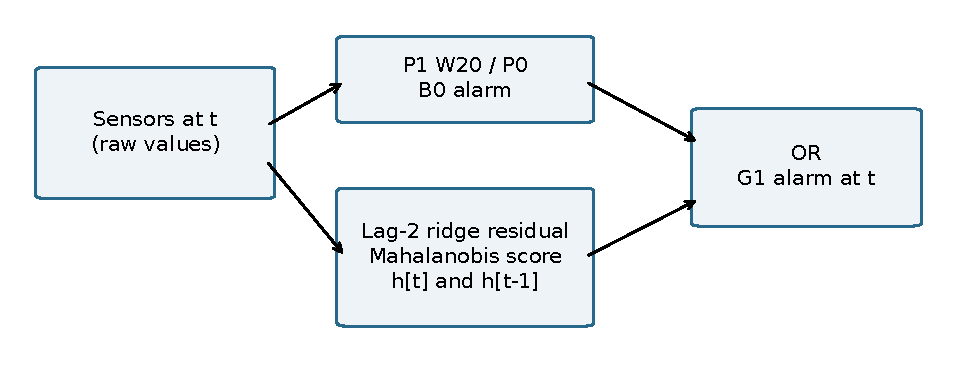
\includegraphics[width=.95\textwidth]{figures/flow.pdf}
\caption{Frozen processing paths. Both paths use data available by the current observation. Only the auxiliary path receives consecutive confirmation; the baseline alarm is preserved. A gap resets residual/gate history but does not reset B0's same-partition 20-row window.}
\label{fig:flow}
\end{figure*}

\section{Evaluation Design and Exposure History}
The G1 round examined three gates (single exceedance G0, consecutive G1, and current exceedance plus either of the previous two for G2) at normal-C quantiles 0.995 and 0.999. The six scores/configurations were calculated before duplicate decisions were flagged. G2 matched G1's binary calibration/selection outputs at each threshold but is a different rule; G0 at 0.999 matched a prior R5 configuration. The selected configuration was G1 at 0.999. A later fixed validation added an old-threshold G1 control, making three observed G1-family configurations in the audit, not three independently selected models.

Selection required pooled S to reduce FN strictly, increase $F_2$ strictly, and not reduce $F_1$. S1 and S2 separately required FN nonincrease and $F_1/F_2$ nondecrease. Each required block also imposed
\begin{equation}
 \Delta\mathrm{FP}\leq\lfloor0.001N_0\rfloor,\qquad
 \mathrm{FP}\leq\lfloor0.01N_0\rfloor.
\end{equation}
Thus S2's 616 normal rows permit zero added FP. The same maintenance conditions apply to V; FN $0\to0$ passes maintenance but FN reduction is \texttt{not\_assessable}. S's strict effect conditions apply again descriptively to H. Integer budgets use exact floor; metric comparisons use tolerance $10^{-12}$. Eligible choices rank by pooled $F_2$, fewer FP, then simpler gate. These are project policies, not official competition rules or validated field-cost ratios.

A preceding 18-candidate study selected none. Its original strict V improvement requirement was impossible when baseline FN was zero and $F_2=1$. Separating improvement from maintenance corrected that policy in the next round, without changing old predictions or rescinding the earlier R5 failure: its S2 FP rose from 6 to 7 and exceeded both budgets. The additional confirmation policy was motivated by that observed development error. It is therefore development on already examined S data, not a single pristine preregistration.

Local historical logs place the G1 selection artifact at 12:53:34 UTC and the subsequent V/H evaluation command at 12:53:55 UTC on 2026-10-04. These records support within-round ordering but are not independent tamper-proof proof. At least four preceding development rounds had already used these same data. The audit identifies no unused unique observation. Copies, replays, 151 earlier regression checks, and 76 later check items do not create new data. No independent new acquisition, significance test, or iid bootstrap is presented.

\section{Results}
\subsection{Aligned Observation-Level Comparison}
Table~\ref{tab:main} is regenerated from stored predictions on identical row IDs and labels. S improves by one detected anomalous row with eight FP retained. S2 remains at three TP and six FP; its FPR is 0.974026\%, close to the 1\% ceiling. V has 90 TP and no errors for both models, confirming maintenance only. H gains 15 detected anomalous rows, with recall increasing from 92.1569\% to 96.3585\% and precision from 99.6970\% to 99.7101\%. Both produce one FP in 3,990 normal rows (0.250627 FP per 1,000 observations). No original B0 detection is lost.

\begin{table*}[t]
\caption{Identical-row B0/G1 comparison. Counts are observations, not independent failures. FPR is percent; precision, recall and F-scores are proportions. S overlaps S1/S2. V and H are reused records, not independent new tests.}
\label{tab:main}\centering\small\begin{tabular}{llrrrrrrrrrrr}
\toprule
Set & Model & $N_0$ & $N_1$ & TP & FN & FP & TN & Prec. & Recall & FPR(\%) & $F_1$ & $F_2$ \\
\midrule
S1 & B0 & 639 & 18 & 15 & 3 & 2 & 637 & 0.8824 & 0.8333 & 0.3130 & 0.8571 & 0.8427 \\
S1 & G1 & 639 & 18 & 16 & 2 & 2 & 637 & 0.8889 & 0.8889 & 0.3130 & 0.8889 & 0.8889 \\
S2 & B0 & 616 & 3 & 3 & 0 & 6 & 610 & 0.3333 & 1.0000 & 0.9740 & 0.5000 & 0.7143 \\
S2 & G1 & 616 & 3 & 3 & 0 & 6 & 610 & 0.3333 & 1.0000 & 0.9740 & 0.5000 & 0.7143 \\
S & B0 & 1255 & 21 & 18 & 3 & 8 & 1247 & 0.6923 & 0.8571 & 0.6375 & 0.7660 & 0.8182 \\
S & G1 & 1255 & 21 & 19 & 2 & 8 & 1247 & 0.7037 & 0.9048 & 0.6375 & 0.7917 & 0.8559 \\
V & B0 & 731 & 90 & 90 & 0 & 0 & 731 & 1.0000 & 1.0000 & 0.0000 & 1.0000 & 1.0000 \\
V & G1 & 731 & 90 & 90 & 0 & 0 & 731 & 1.0000 & 1.0000 & 0.0000 & 1.0000 & 1.0000 \\
H & B0 & 3990 & 357 & 329 & 28 & 1 & 3989 & 0.9970 & 0.9216 & 0.0251 & 0.9578 & 0.9357 \\
H & G1 & 3990 & 357 & 344 & 13 & 1 & 3989 & 0.9971 & 0.9636 & 0.0251 & 0.9801 & 0.9701 \\
\bottomrule
\end{tabular}

\end{table*}

\subsection{Threshold Versus Confirmation}
Table~\ref{tab:controls} holds B0 and the R5 score function fixed. At the selected threshold, G0 on H has FN10/FP4, whereas G1 has FN13/FP1. Confirmation removes three false-positive observations while foregoing three anomalous detections available to G0. Comparing G1 at the old threshold 19.48692067098804 with G1 at the selected threshold isolates an additional two H detections with the same FP count. Neither post-hoc comparison reselects the model. The unconfirmed old-threshold R5 control has FN11/FP3 on H but still fails S2; its favorable pooled H score cannot overturn that failure.

\begin{table}[t]
\caption{H controls on $N_0=3990,N_1=357$. ``New'' means selected $\theta$, not a newly tuned threshold. All controls are post-hoc frozen analyses.}
\label{tab:controls}\centering\small\begin{tabular}{lrrrr}
\toprule
Rule & FN & FP & $F_1$ & $F_2$ \\
\midrule
B0 & 28 & 1 & 0.957787 & 0.935722 \\
G1 & 13 & 1 & 0.980057 & 0.970107 \\
G0, new $\theta$ & 10 & 4 & 0.980226 & 0.975267 \\
G0, old $\theta$ & 11 & 3 & 0.980170 & 0.973551 \\
G1, old $\theta$ & 15 & 1 & 0.977143 & 0.965556 \\
\bottomrule
\end{tabular}

\end{table}

\subsection{What the Added Rows Mean}
H contains 13 contiguous anomalous observation groups. Both systems already detect all 13, so the number of newly discovered whole groups is zero. The 15 added detections occur in three groups. In the earliest affected group, B0 first alarms 0.4 seconds after the first recorded observation and G1 after 0.3 seconds. All 13 groups begin anomalous and are left-censored with respect to physical onset. This 0.1-second change is neither fault-prevention lead time nor a measured delay from actual fault onset.

Normal H contains one false-alarm row and one contiguous false-alarm episode for both models. The sum of normal within-group adjacent observed intervals is 387.2 seconds. Dividing one episode by that span yields 9.2975 per observed hour, but acquisition uptime is unknown: that denominator cannot establish a field hourly alarm rate. We retain the span-normalized diagnostic in the archive and do not count collection gaps as normal operation.

\begin{figure*}[t]
\centering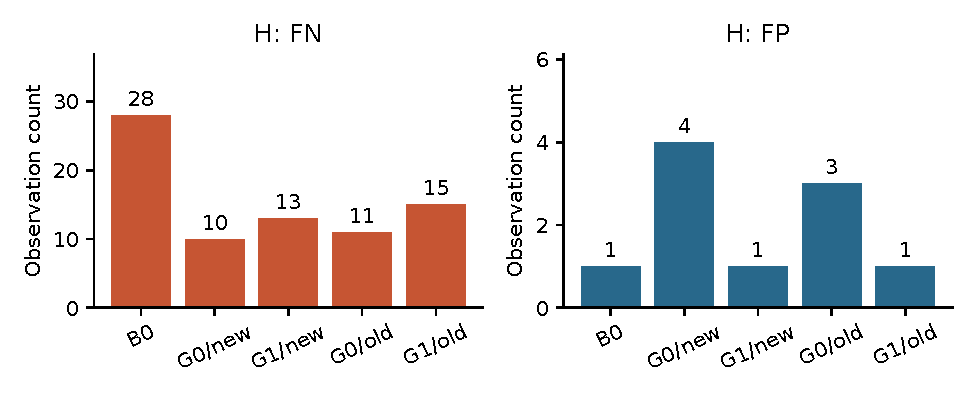
\includegraphics[width=.87\textwidth]{figures/fn_fp_H.pdf}
\caption{H false-negative/false-positive counts for fixed controls. The ordering reflects the registered comparison, not ranking or reselection. Both threshold relaxation and confirmation influence the tradeoff.}
\label{fig:tradeoff}
\end{figure*}

\subsection{Implementation and Reproduction}
The fixed-model record includes batch versus one-observation replay, separate-process model reload, boundary checks, strict ties, and future-sensor perturbations. Core inference hashes agree between selection and frozen validation. The original online helper can treat a nonfinite B0 score as a non-alarm; a later external-input wrapper rejects incomplete sensors instead. Supplied performance data contain no missing values, so this interface correction does not alter their scores. Both source versions and their scope are preserved.

For this manuscript package, a separate fixed-setting reconstruction refits only the two PCA routes and R5 on T, recomputes calibration quantities on normal C, and saves new objects away from selected models. It reproduces selection/H alarms exactly; numerical score comparisons allow $10^{-9}$ absolute and relative tolerance. Stored-prediction metric regeneration agrees within $10^{-12}$. These are computational reproduction checks, not independent performance replications. The package includes all inputs and scripts required for relocation; its validation log distinguishes inherited checks from newly executed checks.

\section{Discussion and Limitations}
The result supports a narrow empirical answer to the research question: in these reused observations, confirmed predictive residuals recover some B0 misses while preserving the observed FP count. It does not establish that the gate limits FP on future operation. The OR architecture prevents lost baseline alarms but can only maintain or increase false positives relative to B0. Confirmation can also discard real short excursions, as the G0 contrast demonstrates.

Three inferential limitations dominate. First, all available unique rows had previous training, calibration, selection, evaluation, or contextual use, and at least four earlier development rounds reused the partitions. The record proves neither the magnitude of selection bias nor its absence. Second, class and date are confounded and actual operating regimes are undocumented. Third, the effect is row coverage within already-detected groups, with unknown physical event independence and onset. A single FP and overlapping windows do not justify a deployment-rate guarantee or a significance claim.

The method combines established building blocks; the archive's detail is not evidence of algorithmic originality. The comparisons isolate the local modification to a chosen baseline, but do not establish broad superiority over modern detectors. Necessary next evidence consists of separately acquired labeled sessions with known operating conditions, held untouched until the pipeline and decision criteria are fixed. Additional same-data searching would not resolve that deficit.

\section{Conclusion}
PCA + R5 prediction-residual auxiliary alarm (G1) preserves a fixed PCA alarm and confirms consecutive one-step residual exceedances. On the exposed H records it reduces FN from 28 to 13 with FP remaining one; later development data show maintenance rather than independently reproduced miss reduction. Controls expose the cost of confirmation, while event analysis prevents interpreting 15 added rows as 15 new failures. The package makes the bounded result reproducible without elevating repeated computation into independent evidence.
\label{mainend}
\clearpage
\section*{Impact Statement}
False reassurance from a monitoring alarm may delay maintenance, while unnecessary alarms may interrupt production. This case study does not demonstrate safe autonomous intervention, reduced downtime, or avoided faults. Use would require independently collected data, verified sensor semantics, and a responsible operational decision process. Authors, affiliations, funding, and conflicts of interest are not established in this anonymous draft and must not be inferred. The study and manuscript were prepared with AI assistance; the accompanying adversarial report is author-side self-review, not external peer review. Data redistribution rights require separate confirmation; this archive is for the user's custody and has not been publicly submitted or deployed.
\bibliography{references}
\bibliographystyle{icml2026}
\clearpage
\appendix
\onecolumn
\section{Complete Reproduction Contract}
The main paper uses the official ICML 2026 default anonymous submission style, without the accepted option. This is a format reference, not a submission or acceptance claim. The Korean companion is an extended research manuscript. Both use the same regenerated tables, figures, model manifest, and observation counts. Archive entry points are described in README.md; selected models are immutable and reconstructed models are written to a new output directory.

The numerical feature order is mean(AI0,AI1,AI2), std(AI0,AI1,AI2), RMS(AI0,AI1,AI2), min(AI0,AI1,AI2), max(AI0,AI1,AI2). Standard deviation uses $ddof=0$. A feature is retained if its normal-T standard deviation exceeds $10^{-12}\max(1,|\mathrm{mean}|)$. Effective PCA rank uses eigenvalues greater than $\max(10^{-12},10^{-10}\lambda_1)$. The chosen $k=2$ is below both route ranks. There is no seed search for deterministic full-SVD PCA or ridge regression. All labels are used only in stored evaluation, selection, or explicitly documented prior supervised calibration, never numerical detector inputs.

\begin{algorithm}[h]
\caption{Selected G1 online update (complete finite inputs)}\label{alg:online}
\begin{algorithmic}[1]
\REQUIRE Frozen B0 routes, R5 scaler/ridge/covariance, $\eta$, $\theta$; prior state
\STATE Receive current timestamp and raw sensor vector $x_t$; reject invalid external inputs.
\IF{new original partition or file/session}
\STATE Clear B0's row window, R5 lag history, and previous exceedance.
\ELSIF{elapsed time from previous observation $>0.5$ seconds}
\STATE Clear R5 lag history and previous exceedance; retain B0's row window.
\ENDIF
\STATE Append $x_t$ to B0's window; use W20 when full, otherwise P0; calculate $b_t$.
\STATE Set $h_t=0$; if two valid preceding observations exist, predict $x_t$, observe its residual and set $h_t=\ind[s_t>\theta]$.
\STATE Emit $g_t=b_t\lor(h_t\land h_{t-1})$ at the current observation time, never retrospectively.
\STATE Update lag history and store current $h_t$; do not reset for a reporting-only S/V block boundary.
\end{algorithmic}
\end{algorithm}

B0's maximum row context is current plus 19 past rows; G1 auxiliary context is current plus three past rows in the same continuity group. Inputs at $t$ are required to score the forecast error at $t$; the prediction can be prepared earlier, but the alarm cannot. Computation latency is distinct from timestamp availability. Physical session metadata were not supplied, so gap groups are only an operational proxy. New-data evaluation requires a provided acquisition-session identifier and rejects interleaved, missing, or nonfinite inputs.

\section{Detailed Metrics and Continuous Scores}
F1 is $2TP/(2TP+FN+FP)$ and F2 is $5TP/(5TP+4FN+FP)$. No field cost ratio is inferred from the coefficient four. Undefined divisions are reported as NA; a normal-only block supports FP/FPR assessment rather than anomaly improvement. Balanced accuracy is mean sensitivity and specificity; MCC uses the four confusion counts. These all derive from the same rows. The continuous score in the main text supports AP, trapezoidal PR-AUC and ROC-AUC, which are not defined by binary predictions. AP uses recall increments weighted by precision, whereas PR-AUC uses trapezoids. Cross-set differences in prevalence prohibit treating AP as a directly comparable standalone ranking across S, V and H.
\begin{table}[!ht]\centering\caption{Supplementary H metrics, same $3990/357$ class denominators.}\begin{tabular}{lrrrrrrrrr}
\toprule
Model & FNR & Spec. & NPV & Acc. & Bal.Acc. & MCC & $F_{0.5}$ & FDR & FOR \\
\midrule
B0 & 0.078431 & 0.999749 & 0.993030 & 0.993329 & 0.960659 & 0.955041 & 0.980918 & 0.003030 & 0.006970 \\
G1 & 0.036415 & 0.999749 & 0.996752 & 0.996779 & 0.981667 & 0.978475 & 0.990213 & 0.002899 & 0.003248 \\
\bottomrule
\end{tabular}
\end{table}
\begin{table}[!ht]\centering\caption{Supplementary S metrics, same $1255/21$ class denominators.}\begin{tabular}{lrrrrrrrrr}
\toprule
Model & FNR & Spec. & NPV & Acc. & Bal.Acc. & MCC & $F_{0.5}$ & FDR & FOR \\
\midrule
B0 & 0.142857 & 0.993625 & 0.997600 & 0.991379 & 0.925384 & 0.766128 & 0.720000 & 0.307692 & 0.002400 \\
G1 & 0.095238 & 0.993625 & 0.998399 & 0.992163 & 0.949194 & 0.794204 & 0.736434 & 0.296296 & 0.001601 \\
\bottomrule
\end{tabular}
\end{table}
\begin{table}[!ht]\centering\caption{Supplementary V metrics, same $731/90$ class denominators.}\begin{tabular}{lrrrrrrrrr}
\toprule
Model & FNR & Spec. & NPV & Acc. & Bal.Acc. & MCC & $F_{0.5}$ & FDR & FOR \\
\midrule
B0 & 0.000000 & 1.000000 & 1.000000 & 1.000000 & 1.000000 & 1.000000 & 1.000000 & 0.000000 & 0.000000 \\
G1 & 0.000000 & 1.000000 & 1.000000 & 1.000000 & 1.000000 & 1.000000 & 1.000000 & 0.000000 & 0.000000 \\
\bottomrule
\end{tabular}
\end{table}
\begin{table}[!ht]\centering\caption{Ranking metrics of the defined continuous operating score. Prevalence differs across sets; these rows do not rank datasets.}\begin{tabular}{lrrrr}
\toprule
Set & Model & AP & PR-AUC & ROC-AUC \\
\midrule
S & B0 & 0.859801 & 0.859735 & 0.875052 \\
S & G1 & 0.906559 & 0.906516 & 0.917473 \\
V & B0 & 1.000000 & 1.000000 & 1.000000 \\
V & G1 & 1.000000 & 1.000000 & 1.000000 \\
H & B0 & 0.987098 & 0.987086 & 0.996203 \\
H & G1 & 0.995770 & 0.995766 & 0.999490 \\
\bottomrule
\end{tabular}
\end{table}
\begin{figure}[h]\centering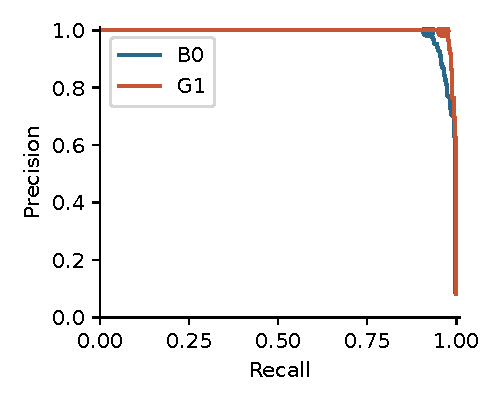
\includegraphics[width=.43\textwidth]{figures/pr_H.pdf}\caption{H precision--recall curves from the explicitly defined continuous operational scores. Dots mark frozen operating points. This is descriptive analysis on reused H, not a threshold search or proof of generalization.}\end{figure}

\clearpage
\section{All Local Candidates and Fixed Controls}
\begin{table}[!ht]\centering\caption{All six follow-up configurations on S. G2 duplicates concern observed C/S binary decisions, not universally equivalent algorithms. Full block-specific failed rules and timings are in the original all\_trials.csv.}\begin{tabular}{lrrrrrr}
\toprule
Rule & $q$ & FN & FP & $F_1$ & $F_2$ & Decision \\
\midrule
G0 & 0.995 & 1 & 14 & 0.7273 & 0.8475 & ineligible \\
G0 & 0.999 & 1 & 9 & 0.8000 & 0.8850 & duplicate \\
G1 & 0.995 & 2 & 9 & 0.7755 & 0.8482 & ineligible \\
G1 & 0.999 & 2 & 8 & 0.7917 & 0.8559 & selected \\
G2 & 0.995 & 2 & 9 & 0.7755 & 0.8482 & duplicate \\
G2 & 0.999 & 2 & 8 & 0.7917 & 0.8559 & duplicate \\
\bottomrule
\end{tabular}
\end{table}
G0 at 0.995 violates S1's FP budget and S2's FP/FPR/F-score conditions. G0 at 0.999 and G1 at 0.995 fail S2's zero-additional-FP budget, absolute FPR, F1 and F2. G2 at 0.995 matches G1 at 0.995 decisions; G2 at 0.999 matches selected G1 decisions and is excluded as redundant on observed data. G0 at 0.999 duplicates prior R5\_A1. Six computed configurations, three rows marked completed, and three duplicate-excluded rows are different accounting units. The broader preceding searches are preserved in the historical CSVs rather than rerun for this paper.
\begin{table}[!ht]\centering\caption{All 18 preceding literature-round candidates on S. None passed its full selection conditions; full failures and unavailable cases are preserved in the CSV. R0 is threshold-only, R1 residual covariance weighting, R2/R3 RBF-SVDD, R4/R5 lag-one/two ridge residuals.}\begin{tabular}{lrrrrr}
\toprule
ID & FN & FP & $F_1$ & $F_2$ & Decision \\
\midrule
R0\_A0 & 3 & 8 & 0.7660 & 0.8182 & not selected \\
R0\_A1 & 3 & 8 & 0.7660 & 0.8182 & not selected \\
R0\_A2 & 3 & 8 & 0.7660 & 0.8182 & not selected \\
R1\_A0 & 3 & 8 & 0.7660 & 0.8182 & not selected \\
R1\_A1 & 3 & 8 & 0.7660 & 0.8182 & not selected \\
R1\_A2 & 3 & 9 & 0.7500 & 0.8108 & not selected \\
R2\_A0 & 3 & 9 & 0.7500 & 0.8108 & not selected \\
R2\_A1 & 3 & 9 & 0.7500 & 0.8108 & not selected \\
R2\_A2 & 3 & 10 & 0.7347 & 0.8036 & not selected \\
R3\_A0 & 3 & 10 & 0.7347 & 0.8036 & not selected \\
R3\_A1 & 3 & 17 & 0.6429 & 0.7563 & not selected \\
R3\_A2 & 3 & 17 & 0.6429 & 0.7563 & not selected \\
R4\_A0 & 2 & 9 & 0.7755 & 0.8482 & not selected \\
R4\_A1 & 2 & 9 & 0.7755 & 0.8482 & not selected \\
R4\_A2 & 2 & 11 & 0.7451 & 0.8333 & not selected \\
R5\_A0 & 1 & 9 & 0.8000 & 0.8850 & not selected \\
R5\_A1 & 1 & 9 & 0.8000 & 0.8850 & not selected \\
R5\_A2 & 1 & 10 & 0.7843 & 0.8772 & not selected \\
\bottomrule
\end{tabular}
\end{table}
\begin{table}[!ht]\centering\caption{Fixed controls on S, $N_0=1255,N_1=21$. Passing pooled S alone is insufficient when S2 fails.}\begin{tabular}{lrrrr}
\toprule
Rule & FN & FP & $F_1$ & $F_2$ \\
\midrule
B0 & 3 & 8 & 0.765957 & 0.818182 \\
G1 & 2 & 8 & 0.791667 & 0.855856 \\
G0, new $\theta$ & 1 & 9 & 0.800000 & 0.884956 \\
G0, old $\theta$ & 1 & 9 & 0.800000 & 0.884956 \\
G1, old $\theta$ & 2 & 8 & 0.791667 & 0.855856 \\
\bottomrule
\end{tabular}
\end{table}
\clearpage
\section{Observation Groups, Coverage, and Time}
\begin{table}[!ht]\centering\caption{All 13 H anomalous groups. Delay $d$ is seconds from first recorded observation, not physical fault onset. Every group is already detected by B0; all are left-censored.}\begin{tabular}{lrrrrrr}
\toprule
Burst & Rows & B0 TP/FN & G1 TP/FN & Added & B0 $d$ & G1 $d$ \\
\midrule
1:9 & 25 & 12/13 & 19/6 & 7 & 0.4 & 0.3 \\
1:10 & 8 & 8/0 & 8/0 & 0 & 0.0 & 0.0 \\
1:11 & 4 & 4/0 & 4/0 & 0 & 0.0 & 0.0 \\
1:12 & 50 & 48/2 & 49/1 & 1 & 0.0 & 0.0 \\
1:13 & 42 & 42/0 & 42/0 & 0 & 0.0 & 0.0 \\
1:14 & 28 & 28/0 & 28/0 & 0 & 0.0 & 0.0 \\
1:15 & 15 & 15/0 & 15/0 & 0 & 0.0 & 0.0 \\
1:16 & 50 & 37/13 & 44/6 & 7 & 0.0 & 0.0 \\
1:17 & 50 & 50/0 & 50/0 & 0 & 0.0 & 0.0 \\
1:18 & 36 & 36/0 & 36/0 & 0 & 0.0 & 0.0 \\
1:19 & 24 & 24/0 & 24/0 & 0 & 0.0 & 0.0 \\
1:20 & 10 & 10/0 & 10/0 & 0 & 0.0 & 0.0 \\
1:21 & 15 & 15/0 & 15/0 & 0 & 0.0 & 0.0 \\
\bottomrule
\end{tabular}
\end{table}
\begin{figure}[h]\centering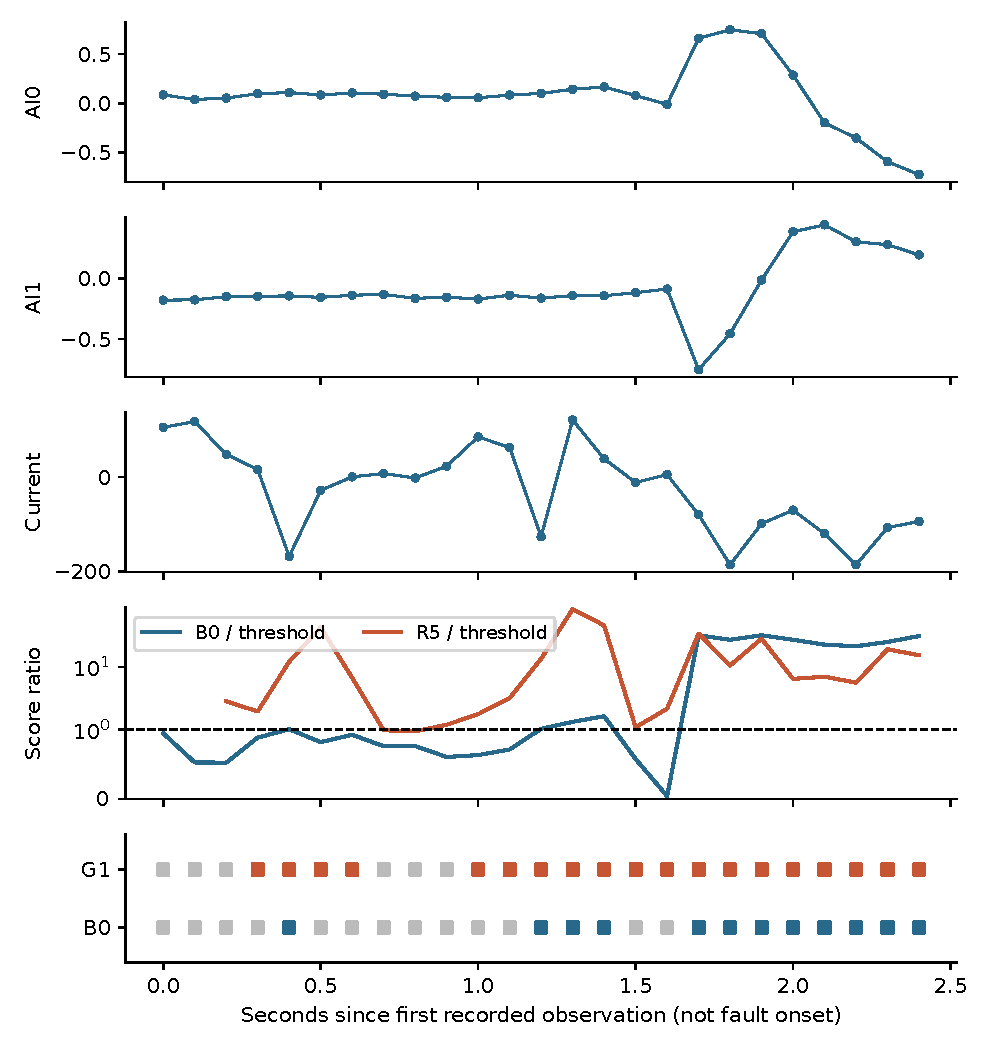
\includegraphics[width=.76\textwidth]{figures/case.pdf}\caption{Earliest chronological H group with additional detections, selected by that fixed descriptive rule. Raw sensor units are undocumented. Gray squares are non-alarms; colored squares are alarms. The complete group is shown; no line crosses an observation gap. The residual is computed after its target arrives. This example illustrates coverage, not a physical cause.}\label{fig:case}\end{figure}
\clearpage
\begin{figure}[t]\centering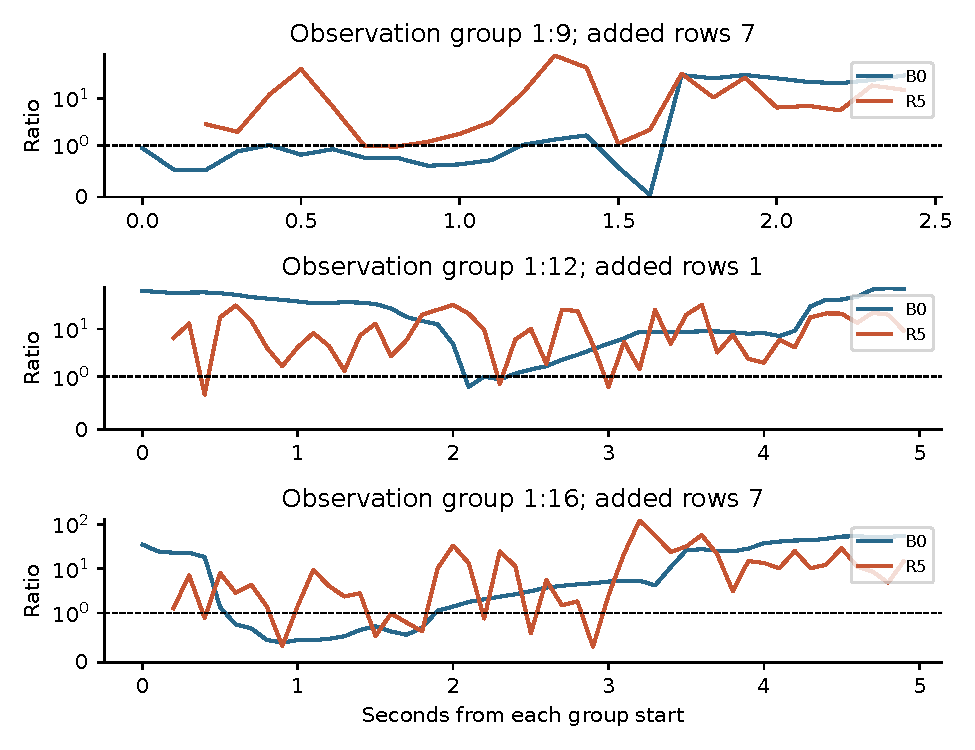
\includegraphics[width=.86\textwidth]{figures/all_affected.pdf}\caption{All three H groups with added detections, on separate elapsed-time axes. No cross-gap line is drawn. No case selection or future context changes the deployed rule.}\end{figure}
\section{Usage, Dependency, and Verification Evidence}
\begin{figure}[h]\centering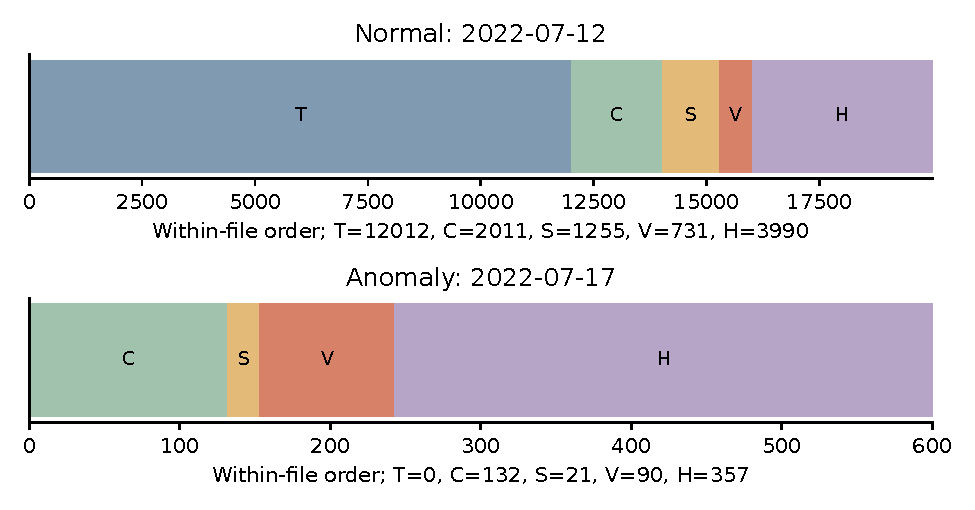
\includegraphics[width=.92\textwidth]{figures/roles.pdf}\caption{Distinct within-file timelines. The two dates are not synchronized. C's anomalous rows belong to historical labeled calibration only; current detector/threshold fitting uses normal T/C. S equals S1 plus S2.}\end{figure}
The audit counts one G1 development/selection round, one frozen-validation round, and at least two full replays. Three G1-family configurations comprise two development thresholds and one old-threshold control. At least four earlier development rounds reused the same S/V/H. A minimum of 106 PCA fitting pipelines across that wider history is not a candidate count: each pipeline includes a spectrum fit and a retained-component fit. The five confirmed R5 fits include two validation-only reconstructions. The 454 reported passing check-item occurrences are $151\times2+76\times2$, with repetitions; they are not 454 models or independent observations. Exact global execution totals remain unknown because local logs are incomplete or overwritten. This manuscript's additional reconstruction and relocation checks occur after that audit cutoff and are logged separately.

The raw originals total 20,600 rows. The duplicate normal row 11566 (CSV line 11567) matches the retained observation at row 11565, including timestamp 2022-07-12 00:43:33.196. All 20,599 unique observations have confirmed prior use, including overlapping input histories; no unused unique record remains in the investigated scope. Unknown per-experiment lineage is not labeled unused. Local hashes establish artifact identity, not retrospective preregistration, and the project lacks a Git commit chronology.

\begin{table}[!ht]\centering\caption{Verification scope. Computational checks do not establish independent data validity.}\begin{tabularx}{\textwidth}{lX}\toprule
Check & Evidence and scope\\\midrule
Fixed model identity & Original B0/R5 SHA-256 manifest; copied objects unchanged.\\
Rows and scores & Same raw row IDs, labels, strict comparisons and alarms; finite numerical tolerance recorded.\\
Causal behavior & Historical future-perturbation tests; online versus batch on full original partitions; no report-boundary reset.\\
Missing input & Original helper limitation recorded; later wrapper rejects invalid external input; no imputation.\\
Training reconstruction & Only frozen two-route PCA and lag-two R5; normal T fit, normal C calibration; exact regenerated alarms.\\
Relocation and documents & Separate extraction/inference and source-to-PDF build logs in verification; checksum and CRC scope explicit.\\
Independent performance & Not performed: no new independent acquisition available.\\\bottomrule\end{tabularx}\end{table}
The user-custody archive includes source, raw and derived data, original registrations, candidate failures, selected models, and a weakness-focused AI-assisted self-review. Some historical inline commands and complete global process histories could not be recovered; these gaps are disclosed rather than reconstructed as original evidence. The self-review is not an external or ICML review. Data rights, authorship, affiliation, funding and conflicts require human confirmation before any public submission.
\end{document}
